\documentclass[11pt, a4paper]{article}

% ── Geometry & Formatting ──
\usepackage[margin=1in]{geometry}
\usepackage{amsmath, amssymb, amsfonts}
\usepackage{booktabs}
\usepackage{graphicx}
\usepackage{xcolor}
\usepackage{tikz}
\usetikzlibrary{calc, positioning, arrows.meta, decorations.pathreplacing, shapes.geometric}
\usepackage{tcolorbox}
\tcbuselibrary{skins, breakable}
\usepackage{enumitem}
\usepackage{hyperref}
\usepackage{fancyhdr}
\usepackage{titlesec}
\usepackage{float}
\usepackage{pifont}
\usepackage{array}

% ── Hyperref Setup ──
\hypersetup{
    colorlinks=true,
    linkcolor=darkblue,
    filecolor=darkblue,
    urlcolor=medblue,
    citecolor=darkgreen,
    pdfauthor={Master Thesis Examination Defense Guide},
    pdftitle={Feature Preprocessing, PCA Dimensionality Reduction, and Eigendecomposition}
}

% ── Color Definitions ──
\definecolor{darkblue}{HTML}{1a365d}
\definecolor{medblue}{HTML}{2b6cb0}
\definecolor{lightblue}{HTML}{ebf8ff}
\definecolor{darkgreen}{HTML}{276749}
\definecolor{lightgreen}{HTML}{f0fff4}
\definecolor{darkred}{HTML}{9b2c2c}
\definecolor{lightred}{HTML}{fff5f5}
\definecolor{darkorange}{HTML}{c05621}
\definecolor{lightorange}{HTML}{fffaf0}
\definecolor{darkpurple}{HTML}{553c9a}
\definecolor{lightpurple}{HTML}{faf5ff}
\definecolor{darkteal}{HTML}{285e61}
\definecolor{lightteal}{HTML}{e6fffa}
\definecolor{lightgray}{HTML}{f7fafc}
\definecolor{bordergray}{HTML}{e2e8f0}

% ── tcolorbox Environments ──
\newtcolorbox{eqbox}[1][]{
    colback=lightpurple, colframe=darkpurple, fonttitle=\bfseries,
    title={#1}, rounded corners, boxrule=1pt, breakable
}
\newtcolorbox{explainbox}[1][]{
    colback=lightblue, colframe=medblue, fonttitle=\bfseries,
    title={#1}, rounded corners, boxrule=1pt, breakable
}
\newtcolorbox{examplebox}[1][]{
    colback=lightgreen, colframe=darkgreen, fonttitle=\bfseries,
    title={#1}, rounded corners, boxrule=1pt, breakable
}
\newtcolorbox{analogybox}[1][]{
    colback=lightorange, colframe=darkorange, fonttitle=\bfseries,
    title={#1}, rounded corners, boxrule=1pt, breakable
}
\newtcolorbox{warningbox}[1][]{
    colback=lightred, colframe=darkred, fonttitle=\bfseries,
    title={#1}, rounded corners, boxrule=1pt, breakable
}
\newtcolorbox{defensebox}[1][]{
    colback=lightteal, colframe=darkteal, fonttitle=\bfseries,
    title={#1}, rounded corners, boxrule=1pt, breakable
}

% ── Header / Footer ──
\setlength{\headheight}{24pt}
\addtolength{\topmargin}{-12pt}
\pagestyle{fancy}
\fancyhf{}
\fancyhead[L]{\small\textcolor{gray}{Thesis Technical Guide: Feature Preprocessing \& PCA}}
\fancyhead[R]{\small\textcolor{gray}{\leftmark}}
\fancyfoot[C]{\thepage}
\renewcommand{\headrulewidth}{0.5pt}

% ── Title Formatting ──
\titleformat{\section}{\color{darkblue}\Large\bfseries}{\thesection}{1em}{}[{\color{medblue}\titlerule[1pt]}]
\titleformat{\subsection}{\color{medblue}\large\bfseries}{\thesubsection}{1em}{}
\titleformat{\subsubsection}{\color{darkteal}\normalsize\bfseries}{\thesubsubsection}{1em}{}

% ── Document ──
\begin{document}

\begin{titlepage}
\centering
\vspace*{0.5cm}
{\Huge \textbf{\color{darkblue}Feature Preprocessing, PCA,\\[0.3em]and Eigendecomposition}}\\[0.6cm]
{\Large \textbf{\color{medblue}Comprehensive Theoretical and Practical Guide for Master's Defense}}\\[1.2cm]

\begin{explainbox}[Document Purpose \& Thesis Context]
This technical reference document provides an exhaustive, mathematically rigorous, and intuitive walkthrough of:
\begin{itemize}[leftmargin=1.2em]
    \item \textbf{Pipeline Technologies:} OpenCV decoding, Float16 + SDPA in V-JEPA~2, and 4-bit NF4 Quantization in Qwen2.5-VL.
    \item \textbf{Frozen-Feature Protocol:} What it means, why it is used, and exact pipeline order.
    \item \textbf{Feature Standardization (StandardScaler):} Formulae, variance distortion prevention, and data leakage safeguards.
    \item \textbf{Linear Algebra Foundations:} Eigenvectors, eigenvalues, characteristic equations, and spectral decomposition of symmetric matrices.
    \item \textbf{Principal Component Analysis (PCA):} Step-by-step mathematical derivation, variance maximization, 95\% variance retention rule, and orthogonal projection.
    \item \textbf{Step-by-Step Worked Numerical Example:} Complete hand calculation showing standardization, covariance matrix, eigenvalue solving, eigenvector normalization, and 1D projection.
    \item \textbf{Architectural Rationale:} Why baseline classifiers require PCA while HAF-STD Net bypasses it.
\end{itemize}
\end{explainbox}

\vspace{1.5cm}
\begin{tabular}{ll}
\textbf{Thesis Focus:} & Action Recognition via Self-Supervised \& Multimodal Foundational Models \\
\textbf{Foundation Models:} & V-JEPA~2.1 (ViT-H, 654M) \& Qwen2.5-VL (7B, 4-bit NF4) \\
\textbf{Datasets:} & FineGym (Sub-action Gymnastics) \& HMDB51 (51 Human Actions) \\
\textbf{Novel Architecture:} & HAF-STD Net (4.8M Trainable Parameters) \\
\end{tabular}

\vfill
{\large \today}
\end{titlepage}

\tableofcontents
\clearpage

% =============================================================================
\section{End-to-End Methodology Timeline \& Key Concepts}
% =============================================================================

To understand where feature preprocessing and PCA fit, we must first map the entire sequential pipeline of the thesis.

\begin{figure}[H]
\centering
\begin{tikzpicture}[
    node distance=0.7cm,
    stage/.style={rectangle, draw=darkblue, fill=lightblue, thick, rounded corners=3pt, text width=13.5cm, minimum height=1.0cm, font=\small},
    model/.style={rectangle, draw=darkpurple, fill=lightpurple, thick, rounded corners=3pt, text width=6.3cm, minimum height=1.0cm, font=\small, text centered},
    arrow/.style={-{Stealth[scale=1.1]}, thick, color=darkblue}
]
    \node[stage] (s1) {\textbf{Stage 1: Raw Video Acquisition} \\ FineGym (1,200 sampled clips $\to$ 272 valid) \& HMDB51 (6,754 clips from HuggingFace).};
    \node[stage, below=of s1] (s2) {\textbf{Stage 2: Video Decoding \& Frame Extraction (OpenCV)} \\ Uniform temporal sampling ($T=8$ for V-JEPA~2, $T=4$ for Qwen) $\to$ Resize $224\times 224$ $\to$ RGB.};
    \node[stage, below=of s2] (s3) {\textbf{Stage 3: Feature Extraction (FROZEN BACKBONES)} \\ Forward pass only with $\nabla_{\mathbf{\Theta}} \mathcal{L} = \mathbf{0}$. No backward pass, no gradient storage.};
    
    \node[model, below left=0.5cm and -0.2cm of s3.south] (m1) {\textbf{V-JEPA~2 (ViT-Huge, 654M)}\\Float16 + SDPA, 8 frames $\to 1{,}280$-d\\(Multi-layer: 4 layers $\times 8$ frames)};
    \node[model, below right=0.5cm and -0.2cm of s3.south] (m2) {\textbf{Qwen2.5-VL (7B)}\\4-bit NF4 Quantization, 4 frames $\to 3{,}584$-d\\(Single mean-pooled representation)};
    
    \node[stage, below=2.3cm of s3] (s4) {\textbf{Stage 4: Dataset Splitting (80\% Train / 20\% Eval)} \\ Strict stratification done \textbf{BEFORE} fitting any normalizer to prevent data leakage.};
    \node[stage, below=of s4] (s5) {\textbf{Stage 5: Feature Preprocessing (StandardScaler)} \\ Compute $\mu_j$ and $\sigma_j$ strictly on 80\% Train $\to$ Transform Train and Test splits.};
    
    \node[stage, below=of s5, fill=lightgreen, draw=darkgreen] (s6a) {\textbf{Branch A: PCA Dimensionality Reduction (For Baseline Classifiers)} \\ 95\% Variance Retention $\to$ Decorrelate features $\to$ 8 Baseline Classifiers (SVM, RF, MLPs).};
    \node[stage, below=of s6a, fill=lightorange, draw=darkorange] (s6b) {\textbf{Branch B: Direct Full-Tensor Routing (For HAF-STD Net)} \\ \textbf{Bypasses PCA} $\to$ Retains $(B, K=4, T=8, D=1280)$ for Haar Wavelet \& Cross-Layer Attention.};

    \draw[arrow] (s1) -- (s2);
    \draw[arrow] (s2) -- (s3);
    \draw[arrow] (s3) -| (m1);
    \draw[arrow] (s3) -| (m2);
    \draw[arrow] (m1) |- (s4);
    \draw[arrow] (m2) |- (s4);
    \draw[arrow] (s4) -- (s5);
    \draw[arrow] (s5) -- (s6a);
    \draw[arrow] (s5) to[out=0,in=0,looseness=1.5] (s6b);
\end{tikzpicture}
\caption{Sequential timeline of the thesis methodology, showing where frozen extraction, data splitting, standardization, PCA, and classifier training occur.}
\end{figure}

\subsection{Why OpenCV and How it Works}

\begin{explainbox}[Technical Mechanics of OpenCV \texttt{VideoCapture}]
\textbf{Why OpenCV?}
Raw video files are not arrays of pixels; they are compressed binary containers (e.g., MP4, AVI, MKV) encoding temporal bitstreams (such as H.264/AVC, H.265/HEVC, or VP9). Deep neural networks cannot consume MP4 files directly; they require normalized tensor representations:
$$\mathbf{X} \in \mathbb{R}^{T \times 3 \times H \times W}$$
OpenCV (Open Source Computer Vision Library) is chosen for its fast C++ backend, hardware-accelerated FFmpeg bindings, and robust demuxing capabilities.

\textbf{How \texttt{VideoCapture} Works Under the Hood:}
\begin{enumerate}[leftmargin=1.2em]
    \item \textbf{Container Demuxing:} OpenCV reads container headers (e.g., MP4 atom box) to parse stream metadata (duration, container framerate $FPS$, total frame count $N_{\text{total}}$, aspect ratio).
    \item \textbf{Bitstream Decoding:} It feeds compressed I-frames (Intra, keyframes), P-frames (Predicted), and B-frames (Bi-directional) into an FFmpeg codec decoder, decompressing Macroblocks/Transform blocks into uncompressed planar YUV420 pixel matrices.
    \item \textbf{Color Conversion:} Raw video frames are decoded into BGR (Blue-Green-Red) byte buffers in host RAM ($H \times W \times 3$, unsigned 8-bit integers $\in [0, 255]$). OpenCV performs colorspace conversion from BGR to RGB:
    $$\text{RGB}_{i,j} = \text{BGR}_{i,j}[2, 1, 0]$$
    \item \textbf{Uniform Temporal Subsampling:} To capture the full motion progression of an action duration without processing thousands of redundant 30~fps frames, uniform time indexing selects $T$ equidistant timestamps:
    $$t_k = \left\lfloor k \cdot \frac{N_{\text{total}} - 1}{T - 1} \right\rfloor, \quad k \in \{0, 1, \ldots, T-1\}$$
    where $T=8$ for V-JEPA~2 and $T=4$ for Qwen2.5-VL.
    \item \textbf{Bicubic Spatial Resizing:} Each sampled frame is interpolated to the canonical resolution $224 \times 224$ pixels required by the Vision Transformer patch embedding projection layer.
\end{enumerate}
\end{explainbox}

\subsection{Why Float16 and SDPA in V-JEPA~2}

\begin{explainbox}[V-JEPA~2 Computational Optimizations]
V-JEPA~2 uses a massive \textbf{Vision Transformer Huge (ViT-H)} architecture containing \textbf{654 million parameters} across 32 transformer blocks, with an internal hidden dimension of $D=1{,}280$.

\textbf{1. What is Float16 (Half Precision)?}
Standard single-precision floating point (FP32) uses 32 bits per weight: 1 sign bit, 8 exponent bits, and 23 mantissa bits (4 bytes). Float16 (FP16) uses 16 bits: 1 sign bit, 5 exponent bits, and 10 mantissa bits (2 bytes).
\begin{itemize}[leftmargin=1.2em]
    \item \textbf{VRAM Reduction:} Storing 654M weights in FP32 requires $\approx 2.62\text{ GB}$, plus activations. In FP16, weight footprint drops by $50\%$ to $\approx 1.31\text{ GB}$.
    \item \textbf{Tensor Core Throughput:} Modern GPUs feature dedicated Tensor Cores that execute FP16 matrix multiplications at $4\times$ to $8\times$ the FLOPS rate of standard FP32 units.
\end{itemize}

\textbf{2. What is SDPA (Scaled Dot-Product Attention)?}
Standard attention computed in naive PyTorch:
$$\text{Attention}(\mathbf{Q}, \mathbf{K}, \mathbf{V}) = \text{softmax}\left(\frac{\mathbf{Q}\mathbf{K}^\top}{\sqrt{d_k}}\right)\mathbf{V}$$
requires materializing the intermediate attention affinity matrix $\mathbf{S} = \mathbf{Q}\mathbf{K}^\top \in \mathbb{R}^{B \times H \times N_{\text{tokens}} \times N_{\text{tokens}}}$ into GPU High-Bandwidth Memory (HBM). For high-resolution video tokens ($N_{\text{tokens}} = 8 \text{ frames} \times 14 \times 14 = 1{,}568$ tokens per clip), materializing $\mathbf{S}$ across 16 attention heads incurs $O(N^2)$ memory allocations and massive memory bandwidth bottlenecks.

\texttt{torch.nn.functional.scaled\_dot\_product\_attention} (SDPA) implements \textbf{FlashAttention-2}:
\begin{itemize}[leftmargin=1.2em]
    \item It tiles queries, keys, and values into small chunks that fit entirely within ultra-fast GPU on-chip SRAM cache ($20\text{ TB/s}$ bandwidth vs $1\text{ TB/s}$ HBM).
    \item It calculates softmax online using running max and sum accumulators without ever writing the large $1{,}568 \times 1{,}568$ attention matrix back to global VRAM.
    \item This achieves a $3\times-5\times$ speedup and reduces attention memory complexity from $O(N^2)$ to $O(N)$.
\end{itemize}
\end{explainbox}

\subsection{What is 4-bit NF4 Quantization in Qwen2.5-VL?}

\begin{explainbox}[Quantization Mechanics: NormalFloat4 (NF4)]
\textbf{The Problem:} Qwen2.5-VL is a 7-Billion parameter Multimodal Large Language Model. Storing 7B parameters in 16-bit precision requires:
$$\text{RAM} = 7 \times 10^9 \times 2 \text{ bytes} \approx 14.0\text{ GB}$$
Running inference with 14 GB of weights plus dynamic KV-caches and visual patch embeddings would exceed standard single-GPU VRAM limits (e.g., 16 GB GPUs) or leave zero memory for feature tensors.

\textbf{What is NF4?}
NormalFloat4 is an information-theoretically optimal non-linear 4-bit data type developed by Dettmers et al. (QLoRA):
\begin{itemize}[leftmargin=1.2em]
    \item Pretrained deep neural network weights follow a zero-mean normal distribution: $\mathbf{W} \sim \mathcal{N}(0, \sigma^2)$.
    \item Standard linear integer quantization (INT4) divides the interval $[-1, 1]$ into 16 evenly spaced bins. However, normally distributed weights have high density near 0 and very few values in the tails. Uniform bins waste precision on empty tail regions and cause high quantization error near zero.
    \item NF4 assigns exact quantiles of the theoretical normal distribution $q_i = \Phi^{-1}(p_i)$ to each of the 16 available 4-bit codes ($2^4 = 16$ discrete values). Every quantization bin has equal empirical probability of containing weights!
    \item \textbf{Result:} Qwen2.5-VL's 14 GB footprint shrinks to $\approx 3.9\text{ GB}$ in VRAM, allowing the 7B model to run frozen feature extraction smoothly with near-zero loss in representational accuracy.
\end{itemize}
\end{explainbox}

\subsection{What are Frozen Features and When Does Freezing Occur?}

\begin{defensebox}[Concept Definition: Frozen-Feature Protocol]
\textbf{What does ``Frozen'' mean?}
A model is ``frozen'' when all its internal learned parameters (weights $\mathbf{W}$ and biases $\mathbf{b}$) are set to read-only during downstream evaluation:
$$\mathbf{\Theta} = \mathbf{\Theta}_{\text{pretrained}}, \quad \text{requires\_grad} = \text{False}, \quad \nabla_{\mathbf{\Theta}} \mathcal{L} = \mathbf{0}$$
When video frames are passed through the network, PyTorch evaluates the model in \texttt{with torch.no\_grad():} mode. No activation computation graph is saved, and no backpropagation gradients are propagated into the backbone.

\textbf{At what step does it occur?}
Freezing is active during \textbf{Stage 3 (Feature Extraction)}. The model acts strictly as a static mathematical transformation:
$$f: \mathbb{R}^{T \times 3 \times 224 \times 224} \longrightarrow \mathbb{R}^D$$
Once all video clips are processed through the backbone, the outputs are stored as fixed numerical arrays on disk. The foundation backbones (V-JEPA~2 and Qwen2.5-VL) are then completely unloaded from GPU memory!

\textbf{Timeline Clarification:}
Feature preprocessing (StandardScaler and PCA) happens \textbf{AFTER} feature extraction, operating purely on the saved feature arrays $\mathbf{Z} \in \mathbb{R}^{N \times D}$.
\end{defensebox}

\clearpage

% =============================================================================
\section{Feature Preprocessing: StandardScaler}
% =============================================================================

\subsection{Why Feature Preprocessing is Mandatory}

Raw feature vectors extracted from deep neural networks have dimensions with vastly differing numerical magnitudes:
\begin{itemize}[leftmargin=1.2em]
    \item Certain latent dimensions might vary between $[-0.01, +0.01]$, while other dimensions (especially after unnormalized layers or residual sums) might range from $[-15.0, +25.0]$.
    \item If unstandardized features are passed directly to PCA, PCA's variance maximization will mistake dimension 2 as being ``2,500 times more informative'' than dimension 1, purely due to arbitrary unit scaling!
    \item Furthermore, distance-based classifiers (SVM with RBF kernel, KNN) compute Euclidean distances $\|\mathbf{x}_i - \mathbf{x}_j\|^2 = \sum_k (x_{ik} - x_{jk})^2$. A feature with scale 20 will completely dominate a feature with scale 0.01, effectively blinding the classifier to the smaller feature.
\end{itemize}

\subsection{Mathematical Formulation}

Let the extracted feature matrix from the training set be $\mathbf{Z}_{\text{train}} \in \mathbb{R}^{N_{\text{train}} \times D}$, where $N_{\text{train}}$ is the number of video training samples and $D$ is the embedding dimension ($D=1{,}280$ for V-JEPA~2, $D=3{,}584$ for Qwen2.5-VL).

\begin{eqbox}[StandardScaler Equations (Eq. 3.18 in Thesis)]
For each feature dimension $j \in \{1, 2, \ldots, D\}$:
\begin{align}
\mu_j &= \frac{1}{N_{\text{train}}} \sum_{i=1}^{N_{\text{train}}} z_{ij} \\[0.5em]
\sigma_j &= \sqrt{\frac{1}{N_{\text{train}} - 1} \sum_{i=1}^{N_{\text{train}}} (z_{ij} - \mu_j)^2} \\[0.5em]
\tilde{z}_{ij} &= \frac{z_{ij} - \mu_j}{\sigma_j}
\end{align}
where:
\begin{itemize}[leftmargin=1.2em]
    \item $\mu_j$ is the sample mean of feature dimension $j$.
    \item $\sigma_j$ is the sample standard deviation (using Bessel's correction $N_{\text{train}}-1$).
    \item $\tilde{z}_{ij}$ is the standardized z-score coordinate, ensuring $\mathbb{E}[\tilde{\mathbf{z}}_j] = 0$ and $\text{Var}(\tilde{\mathbf{z}}_j) = 1$.
\end{itemize}
\end{eqbox}

\subsection{Data Leakage: Why Fit on Train Split Only?}

\begin{warningbox}[Critical Scientific Guardrail: Preventing Data Leakage]
A catastrophic mistake in machine learning evaluation is standardizing the dataset prior to train/test splitting:
$$\mu_{\text{leaked}} = \frac{1}{N_{\text{total}}} \sum_{i=1}^{N_{\text{total}}} z_{ij} \quad \text{\textbf{[INCORRECT / DATA LEAKAGE!]}}$$
If $\mu$ and $\sigma$ are computed across all $N_{\text{total}}$ samples (training + test):
\begin{enumerate}[leftmargin=1.2em]
    \item Information from the test distribution leaks into the training pipeline.
    \item The model is indirectly exposed to the mean, variance, and extreme values of unseen test samples.
    \item This yields artificially inflated test accuracy that collapses in real-world deployment.
\end{enumerate}
\textbf{Correct Protocol Used in Thesis:}
$$\mu_j = \text{mean}(\mathbf{Z}_{\text{train}}[:, j]), \quad \sigma_j = \text{std}(\mathbf{Z}_{\text{train}}[:, j])$$
$$\tilde{\mathbf{Z}}_{\text{train}} = \frac{\mathbf{Z}_{\text{train}} - \boldsymbol{\mu}}{\boldsymbol{\sigma}}, \qquad \tilde{\mathbf{Z}}_{\text{test}} = \frac{\mathbf{Z}_{\text{test}} - \boldsymbol{\mu}}{\boldsymbol{\sigma}}$$
The test set is transformed strictly using the training statistics $\boldsymbol{\mu}$ and $\boldsymbol{\sigma}$. The test set is never inspected during preprocessing parameter estimation.
\end{warningbox}

\clearpage

% =============================================================================
\section{Linear Algebra Foundations: Eigenvectors and Eigenvalues}
% =============================================================================

Before delving into PCA, we must establish complete clarity on eigenvectors and eigenvalues. Examiners frequently probe candidates on these geometric fundamentals.

\subsection{Matrix Multiplication as Geometric Transformation}

A matrix $\mathbf{A} \in \mathbb{R}^{D \times D}$ acts as a linear transformation operator on vectors in $\mathbb{R}^D$. When we multiply $\mathbf{A}\mathbf{x}$:
\begin{itemize}[leftmargin=1.2em]
    \item In general, the resulting vector $\mathbf{y} = \mathbf{A}\mathbf{x}$ has both a \textbf{different length} and points in a \textbf{different direction} (it is rotated and stretched).
\end{itemize}

\begin{figure}[H]
\centering
\begin{tikzpicture}[scale=1.2]
    % Coordinate axes
    \draw[->, thick, gray!60] (-0.5,0) -- (4.2,0) node[right] {$x_1$};
    \draw[->, thick, gray!60] (0,-0.5) -- (0,3.5) node[above] {$x_2$};
    
    % Arbitrary vector x and transformed Ax
    \draw[->, very thick, red] (0,0) -- (1.5, 0.8) node[midway, above left] {$\mathbf{x}$ (ordinary vector)};
    \draw[->, very thick, red!60!black, dashed] (0,0) -- (0.8, 2.2) node[above right] {$\mathbf{A}\mathbf{x}$ (rotated \& stretched)};
    
    % Eigenvector v and transformed Av = lambda v
    \draw[->, very thick, medblue] (0,0) -- (1.8, 1.8) node[midway, below right] {$\mathbf{v}$ (eigenvector)};
    \draw[->, very thick, darkblue] (0,0) -- (3.6, 3.6) node[above right] {$\mathbf{A}\mathbf{v} = \lambda \mathbf{v}$ (pure scaling, NO rotation!)};
\end{tikzpicture}
\caption{Geometric distinction between an arbitrary vector (rotated by $\mathbf{A}$) and an eigenvector (direction invariant, scaled by $\lambda$).}
\label{fig:eigen_intuition}
\end{figure}

\subsection{The Fundamental Eigen-Equation}

\begin{eqbox}[The Eigenvalue Equation]
A non-zero vector $\mathbf{v} \in \mathbb{R}^D$ is an \textbf{eigenvector} of a square matrix $\mathbf{A} \in \mathbb{R}^{D \times D}$ if and only if:
\begin{equation}
\mathbf{A}\mathbf{v} = \lambda \mathbf{v}
\end{equation}
for some scalar $\lambda \in \mathbb{R}$, known as the corresponding \textbf{eigenvalue}.
\end{eqbox}

\begin{explainbox}[Intuitive Meaning of the Equation]
\begin{itemize}[leftmargin=1.2em]
    \item \textbf{Direction Invariance:} The transformation $\mathbf{A}$ does \emph{not} rotate $\mathbf{v}$. The output $\mathbf{A}\mathbf{v}$ lies on the exact same span (line) as $\mathbf{v}$.
    \item \textbf{The Eigenvalue $\lambda$:} Represents the \emph{scaling factor} along that invariant direction:
    \begin{itemize}
        \item If $\lambda > 1$: $\mathbf{v}$ is stretched.
        \item If $0 < \lambda < 1$: $\mathbf{v}$ is compressed.
        \item If $\lambda < 0$: $\mathbf{v}$ is flipped in the opposite direction.
        \item If $\lambda = 0$: $\mathbf{v}$ is collapsed into the origin (lies in the null space of $\mathbf{A}$).
    \end{itemize}
\end{itemize}
\end{explainbox}

\subsection{How to Find Eigenvalues: The Characteristic Equation}

To solve $\mathbf{A}\mathbf{v} = \lambda \mathbf{v}$ algebraically:
\begin{align}
\mathbf{A}\mathbf{v} - \lambda \mathbf{v} &= \mathbf{0} \\[0.3em]
(\mathbf{A} - \lambda \mathbf{I})\mathbf{v} &= \mathbf{0}
\end{align}
where $\mathbf{I}$ is the $D \times D$ identity matrix.

\begin{explainbox}[Why the Determinant Must Equal Zero]
If the matrix $(\mathbf{A} - \lambda \mathbf{I})$ were invertible (non-singular), we could multiply both sides by its inverse:
$$\mathbf{v} = (\mathbf{A} - \lambda \mathbf{I})^{-1} \mathbf{0} = \mathbf{0}$$
This would yield only the trivial solution $\mathbf{v} = \mathbf{0}$. But by definition, an eigenvector \textbf{must be non-zero}!

Therefore, for non-trivial solutions $\mathbf{v} \ne \mathbf{0}$ to exist, the matrix $(\mathbf{A} - \lambda \mathbf{I})$ \textbf{must be singular} (non-invertible). A matrix is singular if and only if its determinant is zero:
\begin{equation}
\det(\mathbf{A} - \lambda \mathbf{I}) = 0
\end{equation}
This determinant equation expands into a degree-$D$ polynomial in $\lambda$, known as the \textbf{Characteristic Polynomial}. The roots of this polynomial are the \textbf{eigenvalues} $\lambda_1, \lambda_2, \ldots, \lambda_D$.
\end{explainbox}

\subsection{Why the Covariance Matrix Guarantees Perfect Properties}

In PCA, we do not perform eigendecomposition on an arbitrary matrix; we perform it specifically on the \textbf{sample covariance matrix} $\mathbf{C} = \frac{1}{N-1} \tilde{\mathbf{Z}}^\top \tilde{\mathbf{Z}}$.

\begin{defensebox}[Three Crucial Properties of the Covariance Matrix]
\textbf{1. Symmetry ($\mathbf{C} = \mathbf{C}^\top$):}
$$\mathbf{C}^\top = \left(\frac{1}{N-1} \tilde{\mathbf{Z}}^\top \tilde{\mathbf{Z}}\right)^\top = \frac{1}{N-1} \tilde{\mathbf{Z}}^\top (\tilde{\mathbf{Z}}^\top)^\top = \frac{1}{N-1} \tilde{\mathbf{Z}}^\top \tilde{\mathbf{Z}} = \mathbf{C}$$
By the \textbf{Spectral Theorem} of linear algebra, any real symmetric matrix has:
\begin{itemize}[leftmargin=1.2em]
    \item Exclusively \textbf{real eigenvalues} (no imaginary numbers).
    \item A complete set of $D$ \textbf{mutually orthogonal eigenvectors}:
    $$\mathbf{v}_i \cdot \mathbf{v}_j = 0 \quad \text{for all } i \ne j$$
\end{itemize}

\textbf{2. Positive Semi-Definiteness ($\mathbf{C} \succeq 0$):}
For any non-zero vector $\mathbf{u} \in \mathbb{R}^D$:
$$\mathbf{u}^\top \mathbf{C} \mathbf{u} = \mathbf{u}^\top \left(\frac{1}{N-1} \tilde{\mathbf{Z}}^\top \tilde{\mathbf{Z}}\right) \mathbf{u} = \frac{1}{N-1} (\tilde{\mathbf{Z}}\mathbf{u})^\top (\tilde{\mathbf{Z}}\mathbf{u}) = \frac{1}{N-1} \|\tilde{\mathbf{Z}}\mathbf{u}\|^2 \ge 0$$
Since the squared Euclidean norm is strictly non-negative, all eigenvalues are guaranteed to be non-negative:
$$\lambda_1 \ge \lambda_2 \ge \cdots \ge \lambda_D \ge 0$$
\textbf{No negative variances exist!}

\textbf{3. Spectral Decomposition:}
Because eigenvectors can be chosen orthonormal ($\mathbf{V}^\top \mathbf{V} = \mathbf{I}$), $\mathbf{C}$ decomposes cleanly as:
$$\mathbf{C} = \mathbf{V} \boldsymbol{\Lambda} \mathbf{V}^\top$$
where $\boldsymbol{\Lambda} = \text{diag}(\lambda_1, \lambda_2, \ldots, \lambda_D)$ is a diagonal matrix containing the eigenvalues, and $\mathbf{V} = [\mathbf{v}_1, \mathbf{v}_2, \ldots, \mathbf{v}_D]$ is an orthogonal matrix whose columns are the eigenvectors.
\end{defensebox}

\clearpage

% =============================================================================
\section{Principal Component Analysis (PCA) Step-by-Step}
% =============================================================================

\subsection{The Core Optimization Goal of PCA}

What is PCA actually trying to do?
\begin{itemize}[leftmargin=1.2em]
    \item Suppose we have a standardized cloud of data points $\tilde{\mathbf{Z}} \in \mathbb{R}^{N \times D}$.
    \item We want to find a unit direction vector $\mathbf{v} \in \mathbb{R}^D$ ($\|\mathbf{v}\| = 1$) such that when we project all data points onto $\mathbf{v}$, the \textbf{variance of the projected points is maximized}.
\end{itemize}

The projection of sample $\tilde{\mathbf{z}}_i$ onto unit vector $\mathbf{v}$ is the scalar $p_i = \tilde{\mathbf{z}}_i \mathbf{v}$. Since the data is zero-mean, the sample variance of the projections is:
$$\text{Var}(p) = \frac{1}{N-1} \sum_{i=1}^N (\tilde{\mathbf{z}}_i \mathbf{v})^2 = \frac{1}{N-1} (\tilde{\mathbf{Z}}\mathbf{v})^\top (\tilde{\mathbf{Z}}\mathbf{v}) = \mathbf{v}^\top \left(\frac{1}{N-1} \tilde{\mathbf{Z}}^\top \tilde{\mathbf{Z}}\right) \mathbf{v} = \mathbf{v}^\top \mathbf{C} \mathbf{v}$$

We formulate the constrained optimization problem using Lagrange multipliers:
$$\max_{\mathbf{v}} \mathcal{L}(\mathbf{v}, \lambda) = \mathbf{v}^\top \mathbf{C} \mathbf{v} - \lambda (\mathbf{v}^\top \mathbf{v} - 1)$$
Taking the derivative with respect to $\mathbf{v}$ and setting it to zero:
$$\frac{\partial \mathcal{L}}{\partial \mathbf{v}} = 2\mathbf{C}\mathbf{v} - 2\lambda \mathbf{v} = \mathbf{0} \implies \mathbf{C}\mathbf{v} = \lambda \mathbf{v}$$
\begin{explainbox}[Profitable Insight: Variance Equals the Eigenvalue]
Notice what happens when we substitute $\mathbf{C}\mathbf{v} = \lambda \mathbf{v}$ back into the variance equation:
$$\text{Variance} = \mathbf{v}^\top \mathbf{C} \mathbf{v} = \mathbf{v}^\top (\lambda \mathbf{v}) = \lambda (\mathbf{v}^\top \mathbf{v}) = \lambda$$
\textbf{Conclusion:}
\begin{itemize}[leftmargin=1.2em]
    \item The direction of maximum variance is the \textbf{eigenvector} $\mathbf{v}_1$ corresponding to the largest eigenvalue $\lambda_1$.
    \item The amount of variance captured along that direction is \textbf{exactly equal to the eigenvalue} $\lambda_1$!
    \item The second principal component $\mathbf{v}_2$ is the eigenvector corresponding to $\lambda_2$ (orthogonal to $\mathbf{v}_1$), capturing variance $\lambda_2$, and so on.
\end{itemize}
\end{explainbox}

\subsection{The Complete 5-Step PCA Algorithm}

\begin{figure}[H]
\centering
\begin{tikzpicture}[
    box/.style={rectangle, draw=medblue, fill=lightblue, thick, rounded corners=3pt, text width=13cm, minimum height=0.9cm, font=\small},
    arr/.style={-{Stealth[scale=1.1]}, thick, color=darkblue}
]
    \node[box] (b1) {\textbf{Step 1: Standardize Features} \\ Center to zero mean and scale to unit variance: $\tilde{\mathbf{Z}} = (\mathbf{Z} - \boldsymbol{\mu}) / \boldsymbol{\sigma}$.};
    \node[box, below=0.5cm of b1] (b2) {\textbf{Step 2: Compute Sample Covariance Matrix} \\ $\mathbf{C} = \frac{1}{N_{\text{train}}-1} \tilde{\mathbf{Z}}_{\text{train}}^\top \tilde{\mathbf{Z}}_{\text{train}} \in \mathbb{R}^{D \times D}$.};
    \node[box, below=0.5cm of b2] (b3) {\textbf{Step 3: Solve Eigendecomposition} \\ $\mathbf{C}\mathbf{v}_j = \lambda_j \mathbf{v}_j \implies \mathbf{C} = \mathbf{V}\boldsymbol{\Lambda}\mathbf{V}^\top$, sorting $\lambda_1 \ge \lambda_2 \ge \cdots \ge \lambda_D \ge 0$.};
    \node[box, below=0.5cm of b3] (b4) {\textbf{Step 4: Select Number of Components ($k^*$) via 95\% Variance Threshold} \\ Find smallest $k$ such that cumulative explained variance ratio $\ge 0.95$.};
    \node[box, below=0.5cm of b4] (b5) {\textbf{Step 5: Project Data onto Lower-Dimensional Subspace} \\ $\mathbf{Z}_{\text{PCA}} = \tilde{\mathbf{Z}} \mathbf{V}_{:k^*} \in \mathbb{R}^{N \times k^*}$.};

    \draw[arr] (b1) -- (b2);
    \draw[arr] (b2) -- (b3);
    \draw[arr] (b3) -- (b4);
    \draw[arr] (b4) -- (b5);
\end{tikzpicture}
\caption{The 5 core algorithmic steps of Principal Component Analysis.}
\end{figure}

\subsection{The 95\% Variance Retention Rule (Eq. 3.20)}

The total variance present across all $D$ standardized features is:
$$\text{Total Variance} = \sum_{j=1}^D \text{Var}(\tilde{\mathbf{z}}_j) = \text{Tr}(\mathbf{C}) = \sum_{j=1}^D \lambda_j = D$$
The \textbf{Explained Variance Ratio (EVR)} of component $j$ is:
$$\text{EVR}_j = \frac{\lambda_j}{\sum_{i=1}^D \lambda_i}$$
The cumulative explained variance retained by keeping the first $k$ components is:
$$\text{CEVR}_k = \frac{\sum_{j=1}^k \lambda_j}{\sum_{i=1}^D \lambda_i}$$

\begin{eqbox}[95\% Variance Cutoff Formula (Eq. 3.20 in Thesis)]
$$k^* = \arg\min_k \left( \frac{\sum_{j=1}^k \lambda_j}{\sum_{i=1}^D \lambda_i} \ge 0.95 \right)$$
We retain exactly the top $k^*$ eigenvectors $[\mathbf{v}_1, \mathbf{v}_2, \ldots, \mathbf{v}_{k^*}] = \mathbf{V}_{:k^*} \in \mathbb{R}^{D \times k^*}$, discarding the remaining $D - k^*$ trailing dimensions.
\end{eqbox}

\subsection{Dimensionality Reduction Results in the Thesis}

\begin{table}[H]
\centering
\caption{Empirical PCA Dimensionality Reduction Results (95\% Variance Threshold).}
\label{tab:pca_results}
\begin{tabular}{lcccc}
\toprule
\textbf{Dataset \& Model} & \textbf{Original Dim ($D$)} & \textbf{Retained Dim ($k^*$)} & \textbf{Dimensionality Reduction} \\
\midrule
\textbf{FineGym (4 classes)} & & & \\
\quad V-JEPA~2 (ViT-H) & $1{,}280$ & $\mathbf{90}$ & $-93.0\%$ \\
\quad Qwen2.5-VL (7B)  & $3{,}584$ & $\mathbf{142}$ & $-96.0\%$ \\
\midrule
\textbf{HMDB51 (51 classes)} & & & \\
\quad V-JEPA~2 (ViT-H) & $1{,}280$ & $\mathbf{286}$ & $-77.7\%$ \\
\quad Qwen2.5-VL (7B)  & $3{,}584$ & $\mathbf{719}$ & $-79.9\%$ \\
\bottomrule
\end{tabular}
\end{table}

\begin{defensebox}[Why did HMDB51 retain more dimensions than FineGym?]
\textbf{Defense Question:} ``Why did PCA retain 286 dimensions for V-JEPA~2 on HMDB51, but only 90 dimensions on FineGym?''

\textbf{Examiner-Ready Answer:}
\begin{itemize}[leftmargin=1.2em]
    \item \textbf{Intrinsic Semantic Complexity:} FineGym evaluates 4 highly structured gymnastic apparatus events (Vault, Uneven Bars, Balance Beam, Floor Exercise). The visual discriminators are tightly clustered around specific apparatus geometry and athlete body orientation, requiring very few principal axes to capture $95\%$ of feature variation.
    \item \textbf{Broad Spectrum of Human Actions:} HMDB51 spans 51 diverse daily, athletic, and combat actions (e.g., \emph{brush hair, catch, climb, draw sword, drink, ride horse, shoot bow, sword}). Distinguishing across 51 diverse semantic clusters requires an intrinsically higher-dimensional manifold ($k^*=286$ and $719$) to preserve subtle motion and object interactions.
\end{itemize}
\end{defensebox}

\clearpage

% =============================================================================
\section{Step-by-Step Worked Numerical Walkthrough}
% =============================================================================

To solidify complete intuition, let us walk through a complete numerical calculation by hand on a 2-dimensional dataset ($N=4$ samples, $D=2$ features).

\subsection{Initial Data Matrix}

Suppose our extracted feature matrix $\mathbf{Z} \in \mathbb{R}^{4 \times 2}$ consists of 4 video clip embeddings:
$$\mathbf{Z} = \begin{bmatrix}
2 & 4 \\
4 & 6 \\
6 & 8 \\
8 & 14
\end{bmatrix}$$
Here, column 1 is Feature 1 ($z_1$) and column 2 is Feature 2 ($z_2$).

\subsection{Step 1: Compute Means and Standard Deviations}

\textbf{For Feature 1 ($j=1$):}
$$\mu_1 = \frac{2 + 4 + 6 + 8}{4} = \frac{20}{4} = 5.0$$
$$\text{Var}_1 = \frac{(2-5)^2 + (4-5)^2 + (6-5)^2 + (8-5)^2}{4-1} = \frac{(-3)^2 + (-1)^2 + (1)^2 + (3)^2}{3} = \frac{9 + 1 + 1 + 9}{3} = \frac{20}{3} \approx 6.667$$
$$\sigma_1 = \sqrt{\frac{20}{3}} \approx 2.582$$

\textbf{For Feature 2 ($j=2$):}
$$\mu_2 = \frac{4 + 6 + 8 + 14}{4} = \frac{32}{4} = 8.0$$
$$\text{Var}_2 = \frac{(4-8)^2 + (6-8)^2 + (8-8)^2 + (14-8)^2}{4-1} = \frac{(-4)^2 + (-2)^2 + (0)^2 + (6)^2}{3} = \frac{16 + 4 + 0 + 36}{3} = \frac{56}{3} \approx 18.667$$
$$\sigma_2 = \sqrt{\frac{56}{3}} \approx 4.320$$

Notice how Feature 2 has nearly \textbf{three times the variance} of Feature 1 in raw units ($18.667$ vs $6.667$). Without StandardScaler, Feature 2 would artificially dominate the analysis!

\subsection{Step 2: Construct Standardized Matrix $\tilde{\mathbf{Z}}$}

Using $\tilde{z}_{ij} = \frac{z_{ij} - \mu_j}{\sigma_j}$:
$$\tilde{\mathbf{Z}} = \begin{bmatrix}
\frac{2-5}{2.582} & \frac{4-8}{4.320} \\[0.4em]
\frac{4-5}{2.582} & \frac{6-8}{4.320} \\[0.4em]
\frac{6-5}{2.582} & \frac{8-8}{4.320} \\[0.4em]
\frac{8-5}{2.582} & \frac{14-8}{4.320}
\end{bmatrix}
\approx \begin{bmatrix}
-1.162 & -0.926 \\[0.2em]
-0.387 & -0.463 \\[0.2em]
+0.387 & 0.000 \\[0.2em]
+1.162 & +1.389
\end{bmatrix}$$

\subsection{Step 3: Compute the Covariance Matrix $\mathbf{C}$}

The sample covariance matrix is:
$$\mathbf{C} = \frac{1}{N-1} \tilde{\mathbf{Z}}^\top \tilde{\mathbf{Z}} = \frac{1}{3} \begin{bmatrix}
\sum \tilde{z}_{i1}^2 & \sum \tilde{z}_{i1}\tilde{z}_{i2} \\[0.3em]
\sum \tilde{z}_{i1}\tilde{z}_{i2} & \sum \tilde{z}_{i2}^2
\end{bmatrix}$$
Because each column was standardized with sample standard deviation ($N-1$ divisor), the diagonal elements are strictly equal to 1.0:
$$C_{11} = 1.0, \quad C_{22} = 1.0$$
Now we compute the cross-correlation $r = C_{12} = C_{21}$:
\begin{align*}
\sum_{i=1}^4 \tilde{z}_{i1}\tilde{z}_{i2} &= (-1.162)(-0.926) + (-0.387)(-0.463) + (0.387)(0.000) + (1.162)(1.389) \\
&= 1.076 + 0.179 + 0.000 + 1.614 = 2.869 \\[0.3em]
C_{12} &= \frac{2.869}{3} \approx 0.956
\end{align*}

Thus, our covariance matrix is:
$$\mathbf{C} = \begin{bmatrix}
1.000 & 0.956 \\[0.2em]
0.956 & 1.000
\end{bmatrix}$$
Notice that $\mathbf{C}$ is symmetric ($C_{12} = C_{21}$) and exhibits high correlation ($r = 0.956$) between the two features.

\subsection{Step 4: Solve the Characteristic Equation for Eigenvalues}

We solve $\det(\mathbf{C} - \lambda \mathbf{I}) = 0$:
$$\det \begin{bmatrix}
1 - \lambda & 0.956 \\
0.956 & 1 - \lambda
\end{bmatrix} = 0$$
Evaluating the $2 \times 2$ determinant:
$$(1 - \lambda)(1 - \lambda) - (0.956)^2 = 0$$
$$(1 - \lambda)^2 - 0.914 = 0$$
$$(1 - \lambda)^2 = 0.914 \implies 1 - \lambda = \pm \sqrt{0.914} = \pm 0.956$$
Solving for $\lambda$:
$$\lambda_1 = 1 + 0.956 = \mathbf{1.956}$$
$$\lambda_2 = 1 - 0.956 = \mathbf{0.044}$$

\begin{explainbox}[Verification of Eigenvalue Properties]
\begin{itemize}[leftmargin=1.2em]
    \item \textbf{Trace Property Check:} $\text{Tr}(\mathbf{C}) = C_{11} + C_{22} = 1 + 1 = 2.0$.
    $$\lambda_1 + \lambda_2 = 1.956 + 0.044 = 2.000 \quad \text{(\textbf{Verified!})}$$
    \item \textbf{Determinant Property Check:} $\det(\mathbf{C}) = (1)(1) - (0.956)^2 = 1 - 0.914 = 0.086$.
    $$\lambda_1 \times \lambda_2 = (1.956)(0.044) = 0.086 \quad \text{(\textbf{Verified!})}$$
    \item \textbf{Explained Variance Ratios:}
    $$\text{EVR}_1 = \frac{1.956}{2.000} = 97.8\%, \qquad \text{EVR}_2 = \frac{0.044}{2.000} = 2.2\%$$
\end{itemize}
\end{explainbox}

\subsection{Step 5: Solve for the Eigenvectors}

\textbf{Finding $\mathbf{v}_1$ for $\lambda_1 = 1.956$:}
$$(\mathbf{C} - \lambda_1 \mathbf{I}) \mathbf{v}_1 = \mathbf{0} \implies \begin{bmatrix}
1 - 1.956 & 0.956 \\
0.956 & 1 - 1.956
\end{bmatrix} \begin{bmatrix} v_{11} \\ v_{12} \end{bmatrix} = \begin{bmatrix} 0 \\ 0 \end{bmatrix}$$
$$\begin{bmatrix}
-0.956 & 0.956 \\
0.956 & -0.956
\end{bmatrix} \begin{bmatrix} v_{11} \\ v_{12} \end{bmatrix} = \begin{bmatrix} 0 \\ 0 \end{bmatrix}$$
This yields the equation:
$$-0.956 v_{11} + 0.956 v_{12} = 0 \implies v_{11} = v_{12}$$
We require unit length $\|\mathbf{v}_1\|^2 = v_{11}^2 + v_{12}^2 = 1$:
$$v_{11}^2 + v_{11}^2 = 1 \implies 2 v_{11}^2 = 1 \implies v_{11} = \frac{1}{\sqrt{2}} \approx 0.7071$$
Thus:
$$\mathbf{v}_1 = \begin{bmatrix} 0.7071 \\[0.2em] 0.7071 \end{bmatrix}$$

\textbf{Finding $\mathbf{v}_2$ for $\lambda_2 = 0.044$:}
$$(\mathbf{C} - \lambda_2 \mathbf{I}) \mathbf{v}_2 = \mathbf{0} \implies \begin{bmatrix}
1 - 0.044 & 0.956 \\
0.956 & 1 - 0.044
\end{bmatrix} \begin{bmatrix} v_{21} \\ v_{22} \end{bmatrix} = \begin{bmatrix} 0 \\ 0 \end{bmatrix}$$
$$\begin{bmatrix}
0.956 & 0.956 \\
0.956 & 0.956
\end{bmatrix} \begin{bmatrix} v_{21} \\ v_{22} \end{bmatrix} = \begin{bmatrix} 0 \\ 0 \end{bmatrix} \implies v_{21} = -v_{22}$$
Normalizing to unit length gives:
$$\mathbf{v}_2 = \begin{bmatrix} -0.7071 \\[0.2em] 0.7071 \end{bmatrix}$$

\textbf{Orthogonality Check:}
$$\mathbf{v}_1 \cdot \mathbf{v}_2 = (0.7071)(-0.7071) + (0.7071)(0.7071) = -0.5 + 0.5 = 0.000 \quad \text{(\textbf{Perfect Orthogonality!})}$$

\subsection{Step 6: Apply 95\% Cutoff and Project Data}

Since $\text{EVR}_1 = 97.8\% \ge 95\%$, the 95\% variance threshold retains \textbf{only $k^* = 1$ component}!
We reduce the data from 2 dimensions to 1 dimension using projection matrix $\mathbf{V}_{:1} = \mathbf{v}_1$:
$$\mathbf{Z}_{\text{PCA}} = \tilde{\mathbf{Z}} \mathbf{v}_1 = \begin{bmatrix}
-1.162 & -0.926 \\[0.2em]
-0.387 & -0.463 \\[0.2em]
+0.387 & 0.000 \\[0.2em]
+1.162 & +1.389
\end{bmatrix} \begin{bmatrix} 0.7071 \\[0.2em] 0.7071 \end{bmatrix}
= \begin{bmatrix}
(-1.162 + -0.926) \times 0.7071 \\[0.2em]
(-0.387 + -0.463) \times 0.7071 \\[0.2em]
(0.387 + 0.000) \times 0.7071 \\[0.2em]
(1.162 + 1.389) \times 0.7071
\end{bmatrix}
= \begin{bmatrix}
\mathbf{-1.476} \\[0.2em]
\mathbf{-0.601} \\[0.2em]
\mathbf{+0.274} \\[0.2em]
\mathbf{+1.804}
\end{bmatrix}$$

\begin{examplebox}[Verifying the Variance of the Projected Data]
Let us check the sample variance of these 1D projected scores:
$$\text{Mean} = \frac{-1.476 - 0.601 + 0.274 + 1.804}{4} = 0.000$$
$$\text{Var}(z_{\text{PCA}}) = \frac{(-1.476)^2 + (-0.601)^2 + (0.274)^2 + (1.804)^2}{3} = \frac{2.179 + 0.361 + 0.075 + 3.254}{3} = \frac{5.869}{3} = \mathbf{1.956}$$
\textbf{The variance of the projected coordinates exactly equals $\lambda_1 = 1.956$!}
We preserved $97.8\%$ of the total information while discarding $50\%$ of the dimensions.
\end{examplebox}

\clearpage

% =============================================================================
\section{Architectural Rationale: Why Baseline Classifiers Use PCA but HAF-STD Net Bypasses It}
% =============================================================================

One of the most critical methodological distinctions in the thesis is:
\begin{itemize}[leftmargin=1.2em]
    \item \textbf{Path 1 (Baseline Classifiers):} Standardized features $\longrightarrow$ \textbf{PCA} (95\% variance) $\longrightarrow$ Classifiers.
    \item \textbf{Path 2 (HAF-STD Net):} Standardized multi-layer temporal features $\longrightarrow$ \textbf{NO PCA (Bypassed)} $\longrightarrow$ HAF-STD Net.
\end{itemize}

\subsection{Why Baseline Classifiers Strictly Require PCA}

\begin{enumerate}[leftmargin=1.5em]
    \item \textbf{Mitigating the Curse of Dimensionality ($N \ll D$):}
    \begin{itemize}
        \item On the FineGym dataset, the total available sample size is $N=272$ video clips.
        \item The raw feature dimension from V-JEPA~2 is $D=1{,}280$, and from Qwen2.5-VL is $D=3{,}584$.
        \item In both cases, $N \ll D$ ($272 < 1280$ and $272 < 3584$). When the number of features exceeds the number of training samples, linear models and shallow MLPs have infinite degrees of freedom to memorize spurious noise patterns rather than generalizable action dynamics.
        \item PCA projects the dimensionality down to $k^*=90$ (V-JEPA) and $k^*=142$ (Qwen), restoring a favorable sample-to-feature ratio ($N > k^*$).
    \end{itemize}

    \item \textbf{Eliminating Multicollinearity:}
    \begin{itemize}
        \item Over-parameterized vision transformers produce highly correlated feature channels across visual tokens.
        \item Multicollinear features destabilize classical classifiers:
        \begin{itemize}
            \item In \textbf{Logistic Regression}, correlated features cause gradient instability and explode weight norms.
            \item In \textbf{Support Vector Machines (SVM-RBF)}, distance metrics become distorted because redundant directions are counted multiple times in Euclidean distance computations.
        \end{itemize}
        \item PCA projects features into an orthogonal coordinate system where all off-diagonal covariances are identically zero ($C_{ij} = 0$ for $i \ne j$), providing perfectly decorrelated inputs.
    \end{itemize}

    \item \textbf{Computational Scalability:}
    \begin{itemize}
        \item Training an SVM with an RBF kernel scales as $O(N^2 \cdot D)$ in memory and between $O(N^2 \cdot D)$ to $O(N^3 \cdot D)$ in time.
        \item Random Forests require evaluating split thresholds across all candidate features at every tree node ($O(N_{\text{trees}} \cdot \sqrt{D} \cdot N \log N)$).
        \item Reducing $D=3{,}584$ to $k^*=142$ yields a $25\times$ speedup during hyperparameter cross-validation and training.
    \end{itemize}
\end{enumerate}

\subsection{Why HAF-STD Net Deliberately Bypasses PCA}

\begin{defensebox}[Core Architectural Defense: Why HAF-STD Net Must Bypass PCA]
\textbf{Defense Question:} ``Why did you apply PCA to your baseline classifiers, but bypass PCA for your proposed HAF-STD Net? Isn't that an unfair or inconsistent comparison?''

\textbf{Examiner-Ready Answer:}
``Bypassing PCA for HAF-STD Net is not an inconsistency; it is a fundamental architectural requirement dictated by the physical nature of temporal signal processing:
\begin{enumerate}[leftmargin=1.2em]
    \item \textbf{Destruction of Spatiotemporal Topology:} PCA requires flattening multidimensional data into a 2D matrix $\mathbf{Z} \in \mathbb{R}^{N \times D_{\text{total}}}$. Doing so treats the temporal axis ($T=8$) and discrete layer depth ($K=4$) as an arbitrary bag of unordered numbers, destroying their temporal sequence and layer hierarchy.
    \item \textbf{Requirement of Continuous Time for Haar DWT:} HAF-STD Net introduces \textbf{Spectral-Temporal Decomposition via Haar Discrete Wavelet Transforms}. Wavelets operate on ordered, continuous time series:
    $$\mathbf{a}_k = \frac{1}{2}(\mathbf{h}_{2t} + \mathbf{h}_{2t+1}), \qquad \mathbf{d}_k = \frac{1}{2}(\mathbf{h}_{2t} - \mathbf{h}_{2t+1})$$
    Haar DWT decomposes high-frequency motion transients from low-frequency body postures. If features had been compressed via PCA, the temporal phase relationships required to compute velocity and acceleration would be destroyed.
    \item \textbf{Internal Dimensionality Reduction via Learned Attention:} HAF-STD Net does not suffer from the curse of dimensionality because it incorporates its own \textbf{12-head cross-layer attention mechanism} and bottleneck projection layers (with 4.8M parameters). It learns \emph{task-specific, non-linear dimensionality reduction} optimized directly by classification loss and label smoothing, which is strictly superior to unsupervised linear variance compression.''
\end{enumerate}
\end{defensebox}

\clearpage

% =============================================================================
\section{Quick Reference \& Examination Defense Cheat Sheet}
% =============================================================================

\begin{table}[H]
\centering
\small
\caption{Comprehensive Formula Summary for Preprocessing and PCA.}
\label{tab:formula_summary}
\begin{tabular}{p{3.8cm}p{5.5cm}p{4.2cm}}
\toprule
\textbf{Concept} & \textbf{Mathematical Formula} & \textbf{Practical Role} \\
\midrule
\textbf{Frozen Forward Pass} &
$\mathbf{z}_i = f(\mathbf{x}_i; \mathbf{\Theta}_{\text{frozen}}), \; \nabla_{\mathbf{\Theta}}\mathcal{L} = \mathbf{0}$ &
Isolates pretrained representation quality without backbone tuning. \\[0.8em]

\textbf{Feature Standardization} &
$\tilde{z}_{ij} = \frac{z_{ij} - \mu_j}{\sigma_j}$ &
Prevents high-scale dimensions from dominating PCA variance. \\[0.8em]

\textbf{Sample Covariance} &
$\mathbf{C} = \frac{1}{N_{\text{train}}-1}\tilde{\mathbf{Z}}_{\text{train}}^\top \tilde{\mathbf{Z}}_{\text{train}}$ &
Quantifies pairwise linear correlations between standardized features. \\[0.8em]

\textbf{Eigen-Equation} &
$\mathbf{C}\mathbf{v}_j = \lambda_j \mathbf{v}_j$ &
Defines invariant projection axes (eigenvectors) and variances (eigenvalues). \\[0.8em]

\textbf{Characteristic Equation} &
$\det(\mathbf{C} - \lambda \mathbf{I}) = 0$ &
Yields degree-$D$ polynomial to calculate eigenvalues $\lambda_j$. \\[0.8em]

\textbf{95\% Variance Rule} &
$k^* = \arg\min_k \left( \frac{\sum_{j=1}^k \lambda_j}{\sum_{i=1}^D \lambda_i} \ge 0.95 \right)$ &
Selects minimum number of components preserving $95\%$ total variance. \\[0.8em]

\textbf{Subspace Projection} &
$\mathbf{Z}_{\text{PCA}} = \tilde{\mathbf{Z}} \mathbf{V}_{:k^*} \in \mathbb{R}^{N \times k^*}$ &
Projects standardized features into decorrelated $k^*$-dimensional subspace. \\
\bottomrule
\end{tabular}
\end{table}

\subsection{Top 5 Defense Questions \& Bulletproof Answers}

\begin{defensebox}[Q1: What does an eigenvector physically represent in PCA?]
\textbf{Answer:} An eigenvector represents an orthogonal direction in the high-dimensional feature space along which the data varies. The first eigenvector points in the direction of greatest variance; each subsequent eigenvector points in the direction of greatest remaining variance orthogonal to all preceding components.
\end{defensebox}

\begin{defensebox}[Q2: What does an eigenvalue physically represent in PCA?]
\textbf{Answer:} An eigenvalue $\lambda_j$ is exactly equal to the numerical variance of the data points when projected onto the corresponding eigenvector $\mathbf{v}_j$. The sum of all eigenvalues equals the total variance of the dataset ($D$ for standardized data).
\end{defensebox}

\begin{defensebox}[Q3: Why must StandardScaler be fitted ONLY on the training split?]
\textbf{Answer:} To prevent data leakage. If test set samples are used to compute the mean and standard deviation, information about the evaluation distribution leaks into the model training pipeline, creating overly optimistic, invalid performance metrics.
\end{defensebox}

\begin{defensebox}[Q4: What is the difference between Float16 and NF4 quantization?]
\textbf{Answer:} Float16 is a 16-bit floating-point format (1 sign, 5 exponent, 10 mantissa bits) that halves memory footprint while retaining dynamic range for standard GPU tensor core operations. NF4 is a 4-bit quantile-based quantization format specifically optimized for normally distributed neural network weights, reducing Qwen2.5-VL from 14 GB to $\approx 3.9$ GB VRAM without significant degradation.
\end{defensebox}

\begin{defensebox}[Q5: What is the decorrelation property of PCA?]
\textbf{Answer:} When features are projected onto the principal components, the resulting covariance matrix of the projected features is strictly diagonal:
$$\text{Cov}(\mathbf{Z}_{\text{PCA}}) = \text{diag}(\lambda_1, \lambda_2, \ldots, \lambda_{k^*})$$
All off-diagonal entries are 0, meaning that every projected dimension is completely linearly uncorrelated with every other dimension.
\end{defensebox}

\end{document}
